\documentclass[14pt, a4paper]{article}
\usepackage[T2A]{fontenc}
\usepackage[utf8]{inputenc}
\usepackage[russian]{babel}
\usepackage[left=3cm, right=1.5cm, top=2cm, bottom=2cm]{geometry}
\usepackage{indentfirst}
\usepackage{microtype}
\usepackage{array}
\usepackage{xcolor}
% \usepackage{times}
\usepackage{tempora}
\usepackage{ulem}
\usepackage{setspace}
\usepackage{amsmath}
\usepackage{booktabs}
\usepackage{graphicx}
\usepackage{float}
\usepackage{listings}
\graphicspath{{reports/figures/}{figures/}}
\lstset{basicstyle=\ttfamily\small, breaklines=true, columns=fullflexible, frame=single, keepspaces=true}
\pagestyle{empty}

\makeatletter
\renewcommand\section{\@startsection {section}{1}{\parindent}%
  {-3.5ex \@plus -1ex \@minus -.2ex}%
  {0.5ex}%
  {\normalfont\Large\bfseries}}
\renewcommand\tableofcontents{%
  \begin{center}\Large\bfseries\contentsname\end{center}%
  \@starttoc{toc}%
}
\renewcommand*\l@section{\@dottedtocline{1}{0em}{1.5em}}
\makeatother

\begin{document}
\onehalfspacing

\begin{center}
    \textbf{ФЕДЕРАЛЬНОЕ ГОСУДАРСТВЕННОЕ АВТОНОМНОЕ ОБРАЗОВАТЕЛЬНОЕ} \\
    \textbf{УЧРЕЖДЕНИЕ ВЫСШЕГО ОБРАЗОВАНИЯ} \\
    \textbf{«МОСКОВСКИЙ АВИАЦИОННЫЙ ИНСТИТУТ} \\
    \textbf{(НАЦИОНАЛЬНЫЙ ИССЛЕДОВАТЕЛЬСКИЙ УНИВЕРСИТЕТ)»}
\end{center}

\begin{center}
    \bfseries Институт №8 «Компьютерные науки и \\
    \bfseries прикладная математика» \\
    \bfseries Кафедра 806 «Вычислительная математика \\
    \bfseries и программирование»
\end{center}

\vspace{3cm}

\begin{center}
    \Large\bfseries Отчет \\
    \vspace{0.5cm}
    \mdseries по лабораторной работе №1.3
\end{center}

\vfill

\noindent
\hfill
\begin{tabular}{ll}
Группа:       & М8О-307Б-21 \\
Студент:      & М. С. Ивченко \\
Преподаватель:& доц. В. В. Киндинова \\
Оценка:       & \underline{\makebox[3cm][c]{}} \\ [0.2cm]
Дата:         & \underline{\makebox[3cm][c]{}}
\end{tabular}

\vfill

\begin{center}
    Москва \\
    2026
\end{center}

\newpage

\setcounter{tocdepth}{2}
\tableofcontents
\newpage

\section*{Тема}
\addcontentsline{toc}{section}{Тема}
Цель данной лабораторной работы -- исследовать итерационные методы решения систем линейных алгебраических уравнений. В работе сравниваются метод простых итераций и метод Зейделя, а также анализируется, как выбранная точность влияет на число шагов до сходимости.

\section*{Задание}
\addcontentsline{toc}{section}{Задание}
Реализовать метод простых итераций и метод Зейделя в виде программы, задавая в качестве входных данных матрицу системы, вектор правых частей и точность вычислений. Используя разработанное программное обеспечение, решить СЛАУ. Проанализировать количество итераций, необходимое для достижения заданной точности.

\section*{Теория}
\addcontentsline{toc}{section}{Теория}
Итерационные методы применяются тогда, когда прямое решение СЛАУ слишком дорого или когда нужна последовательность приближений с контролируемой точностью. Систему $Ax=b$ предварительно приводят к виду
\[
    x = \beta + \alpha x.
\]
Обычно это делают путем выделения диагональной части матрицы. Если $A=D+L+U$, где $D$ -- диагональная часть, $L$ -- нижняя, $U$ -- верхняя, то для метода Якоби
\[
    x^{(k+1)}=D^{-1}(b-(L+U)x^{(k)}).
\]
В этом случае $\beta=D^{-1}b$, а $\alpha=-D^{-1}(L+U)$. Все компоненты нового приближения вычисляются только по значениям предыдущего шага, поэтому порядок вычисления компонент не влияет на результат итерации.

Метод Зейделя использует уже обновленные компоненты текущего шага:
\[
    x_i^{(k+1)}=\frac{1}{a_{ii}}\left(b_i-\sum_{j<i}a_{ij}x_j^{(k+1)}-\sum_{j>i}a_{ij}x_j^{(k)}\right).
\]
За счет немедленного использования новых значений метод Зейделя часто сходится быстрее метода простых итераций, хотя строгая скорость зависит от свойств конкретной матрицы.

Если $\|\alpha\|<1$, то процесс сходится, а апостериорная оценка имеет вид
\[
    \|x^*-x^{(k)}\| \le \frac{\|\alpha\|}{1-\|\alpha\|}\|x^{(k)}-x^{(k-1)}\|.
\]
Это неравенство позволяет остановить итерации без знания точного решения. Для метода Зейделя аналогичная оценка может строиться через матрицу перехода Зейделя. На практике также контролируют невязку $\|Ax^{(k)}-b\|$: если она мала, найденное приближение действительно хорошо удовлетворяет исходной системе.

\begin{lstlisting}[language=Python]
for k in range(1, k_aprior + 1):
    x_cur = b + A.dot(x_prev)
    epsilon_k = np.max(np.abs(x_cur - x_prev)) * alpha / (1 - alpha)
    if epsilon_k <= precision_epsilon:
        break
    x_prev = x_cur
\end{lstlisting}

\section*{Ход лабораторной работы}
\addcontentsline{toc}{section}{Ход лабораторной работы}
Решалась система
\[
A=\begin{pmatrix}
21&1&-8&4\\
-9&-23&-2&4\\
7&-1&-17&6\\
8&8&-4&-26
\end{pmatrix},\qquad
b=(-119,79,-24,-52)^T,
\]
с точностью $\varepsilon=10^{-4}$. Матрица имеет диагональное преобладание, поэтому преобразованная итерационная схема сходится.

\begin{table}[H]
\centering
\begin{tabular}{lccr}
\toprule
Метод & Апост. итераций & Априорная оценка & Решение\\
\midrule
Простые итерации & 17 & 65 & $(-6.0000,-1.0000,-1.0000,0.0000)$\\
Зейдель & 10 & 65 & $(-6.0000,-1.0000,-1.0000,0.0000)$\\
\bottomrule
\end{tabular}
\caption{Сравнение количества итераций при $\varepsilon=10^{-4}$.}
\end{table}

\begin{figure}[H]
    \centering
    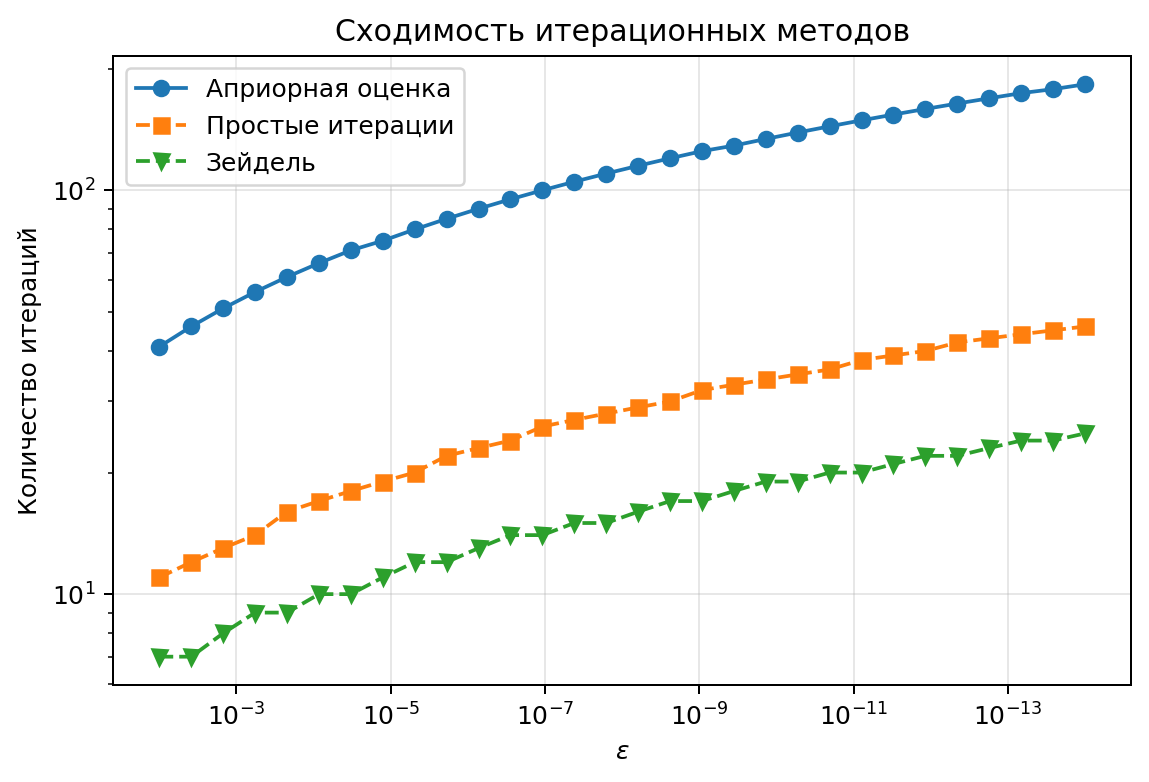
\includegraphics[width=0.86\textwidth]{lab1_3_convergence.png}
    \caption{Зависимость числа итераций от требуемой точности.}
\end{figure}

\section*{Выводы}
\addcontentsline{toc}{section}{Выводы}
Оба итерационных метода сошлись к одному решению, но метод Зейделя потребовал меньше итераций: 10 против 17. Априорная оценка оказалась заметно завышенной, что хорошо видно на графике для разных значений $\varepsilon$.

\end{document}
